\section{A Picard Iteration for the \MA equation}

For quasilinear PDEs such as $\nabla \cdot (A(u) \nabla u ) = f$ it is common to determine the solution via a fixed point iteration. The key aspect lies in a decoupling of the coefficient matrix $A(u)$ and $\nabla u$. Hence, one solves the equations
\[
	\nabla \cdot (A(u^{i} )\nabla u^{i+1}) = f  \text{ and } \nabla \cdot (A(u^{i+1}) \nabla u^{i}) = f, \text{ respectively}
\] 
iteratively.

In this spirit we want to decouple the derivates in the \MA equation. Recall, the \MA equation states
\begin{align}
 \mydet{D^2 u} &= f \nonumber \\
 	\dxx{x_1} u \dxx{x_2} u -\dxy {x_1}{x_2} u \dxy{x_2}{x_1} u  &= f. \label{eq:mongeAmpere detForm}
\end{align}
To shorten and facilitate terms we will denote $x \in \Omega \subset {\R^2} $ by $(x,y)^t$ and the partial derivates with subscripts as for example $\dxx{x_1} u = u_{xx} =  u_{x_1^2}  = u_{x_1 x_1}$.

At first, we multiply \eqref{eq:mongeAmpere detForm} by $-2$ \todo{choose one}
\begin{align}
 	-\dyy u {x} \dyy u {y}-\dyy u {x} \dyy u {y} -\dyx u {x}{y} \dyx u{y}{x} -\dyx u {x}{y} \dyx u{y}{x} &=-2 f. \\
 	-2\dyy u {x} \dyy u {y}-2\dyx u {x}{y} \dyx u{y}{x}  &=-2 f
\end{align}

\subsection*{first try}
Decoupling into the two functions $v = u ,w = u$ we have
\begin{align}
	-w_{yy} v_{xx}-w_{xx} v_{yy} + w_{yx} v_{xy} + w_{xy} v_{yx} = -2f \qquad \textnormal{ on } \Omega \label{eq:decoupled PDE start}
\end{align}
We want to write this equation in divergence form, assuming that $w$ and $v$ are smooth it holds
\begin{align}
	-\nabla \cdot \begin{pmatrix} w_{yy} v_x \\ w_{xx} v_y \end{pmatrix} + w_{yyx}v_x + w_{xxy}v_y
	 +\nabla \cdot \begin{pmatrix} w_{xy} v_y \\ w_{yx} v_x \end{pmatrix}  - w_{xyx}v_y +  w_{yxy}v_x 
	 = -2f.
\end{align}
\todo{vielleicht ein Komma in den zeilenvektor}
Rewriting these terms by matrix products yields 
\begin{align}
%      -&\nabla \cdot \left( \begin{pmatrix} w_{yy} & 0 \\ 0 & w_{xx} \end{pmatrix} \nabla v \right) + (w_{yyx}v_x + w_{xxy}v_y) \nonumber \\
%	 &+\nabla \cdot \left( \begin{pmatrix} 0 & w_{xy}  \\ w_{yx} & 0 \end{pmatrix}  \nabla v \right)  - (w_{xyx}v_y +  w_{yxy}v_x ) 
%	 = -2f \\ 
	       -&\nabla \cdot \left( \begin{pmatrix} w_{yy} & -w_{xy}  \\ -w_{yx} & w_{xx} \end{pmatrix} \nabla v \right) +  \begin{pmatrix} w_{yyx}-w_{yxy} & -w_{xxy} w_{xyx} \end{pmatrix} \nabla v  = -2f  \label{eq:long formula}
\end{align}
We see that the divergence coefficient matrix in \eqref{eq:long formula} is the cofactor matrix of the hessian (Definition \ref{def: cof matrix}) and the right term contains the matrix divergence of the hessian's cofactor matrix leading to
\begin{align}
	-\nabla \cdot \left( \mycof {D^2 w } \nabla v \right) + \nabla \cdot \left(\mycof {D^2 w }\right) \nabla v = -2f.
\end{align}
\todo{ second divergence term}
The cofactor matrix is divergence free (Lemma \ref{la: divergence free cof}) and hence we find a term similar to the linearisation of the \MA equation
\begin{align}
	- \nabla \cdot \left( \mycof{ D^2 w} \nabla v \right)  = -2f.  \label{eq:decoupled PDE}
\end{align}
For a fixed $w$ the left-hand side now is quasilinear in $v$ opposed to the nonlinearity in $u$ in the original PDE. From its derivation it is clear that for smooth functions $w=u, v=u$ \eqref{eq:decoupled PDE} is equivalent to the classical formulation of the \MA equation. Furthermore due to the symmetry of \eqref{eq:decoupled PDE start} in $v$ and $w$ analogously the equation 
\begin{align}
	- \nabla \cdot \left( \mycof{ D^2 v} \nabla w \right)  = -2f.  \label{eq:decoupled PDE2}
\end{align}
can be deduced.

Thus, it is natural to examine the fixed point iteration
\begin{align}
	- \nabla \cdot \left( \mycof{ D^2 u^i} \nabla u^{i+1} \right)  = -2f  \label{eq:decoupled PDE}
\end{align}
for its applicability for numerical schemes approximating a \MA solution.

\subsection*{second try}
Decoupling and not dividing by $-1 $ into the two functions $v = u ,w = u$ and reordering terms we have
\begin{align}
	w_{yy} v_{xx}- w_{xy} v_{yx} - w_{yx} v_{xy} +w_{xx} v_{yy} = 2f \qquad \textnormal{ on } \Omega
\end{align}
Rewriting this by matrix frobenius product yields to
\begin{align}
 \begin{pmatrix} w_{yy} & -w_{xy}  \\ -w_{yx} & w_{xx} \end{pmatrix}: \begin{pmatrix} v_{xx} & v_{yx}  \\  v_{xy} & v_{yy} \end{pmatrix} = 2f.
\end{align}
We see that the left matrix is the cofactor matrix of the hessian (Definition \ref{def: cof matrix}) and the right one the hessian itself and find
\begin{align}
		\mycof {D^2 w }:D^2 v  = 2f  \label{eq:short formula}
\end{align}

???????????????????????????????? \\
Integrating over $\Omega$ and applying integration by parts (Lemma \ref{la: integration by parts Frobenius})we get
\begin{align}
		\int_{\Omega} D^2 v:\mycof {D^2 w }  &= 2f \\
		-\int_{\Omega} \left( \nabla \cdot \mycof {D^2 w } \right) \nabla v + \int_{\partial \Omega} \mycof {D^2 w } \nabla v \mathbf{n} &= 2f
\end{align}
????????????????????????????????


Substituting the identity of Lemma \ref{la: An application of the divergernce product rule} we find
\begin{align}
	\nabla \cdot \left( \mycof {D^2 w } \nabla v \right) = 2f.
\end{align}
Multiplying by $-1$ we get a term the equation
\begin{align}
	- \nabla \cdot \left( \mycof{ D^2 w} \nabla v \right)  = -2f.  \label{eq:decoupled PDE}
\end{align}
For a fixed $w$ the left-hand side now is (at least) quasilinear in $v$ opposed to the nonlinearity in $u$ in the original PDE. From its derivation it is clear that for smooth functions $w=u, v=u$ \eqref{eq:decoupled PDE} is equivalent to the classical formulation of the \MA equation. Furthermore due to the symmetry of \eqref{eq:decoupled PDE start} in $v$ and $w$ analogously the equation 
\begin{align}
	- \nabla \cdot \left( \mycof{ D^2 v} \nabla w \right)  = -2f.  \label{eq:decoupled PDE two}
\end{align}
can be deduced.

Thus, it is natural to examine the fixed point iteration
\begin{align}
	\begin{split}
	- \nabla \cdot \left( \mycof{ D^2 u^i} \nabla u^{i+1} \right)  &= -2f  \text{ in } \Omega \\
		u^{i+1} &= g \textnormal{ on } \partial \Omega
	\label{eq:fixed point iteration}
	\end{split}
\end{align}
for its applicability for numerical schemes approximating a \MA solution.

In \cite{Awanou2014} Awanou analysed the similar iteration process
\begin{align*}
	\nabla \cdot \left( \cof(D^2 u^0) \nabla u^{i+1} \right) &= \nabla \cdot \left( \cof(D^2 u^0) \nabla u^{i} \right) + f - \operatorname{det} (D^2u^i) \textnormal{ in } \Omega, \\
	u^{i+1} &= g \textnormal{ on } \partial \Omega
\end{align*}
showing convergence for the analytical solution $u$ and a sufficent close $u^0$. While Awanou uses a finite difference scheme to solve the PDE in every step we want to exploit the benefits of a DG method and solve every intermediate step by a SIPG method. 

\section{SIPG formulation of the Iteration}\label{sec: SIPG}
Since in every iteration \eqref{eq:fixed point iteration} states a generalised poisson equation we can apply the derived  method of section \ref{sec: SIPG} directly: Given $u^i_h$ find $u^{i+1}_h \in \mathcal P^k_h$ satisfying
\begin{align}
 &\int_{\Omega} \nabla v \cdot \cof(D_h^2 u^{i}) \nabla u_h^{i+1}\\
 & -\sum\limits_{e \in \bigEps^i}\int_{e} \jump {v \average { \cof(D_h^2 u^{i}) \nabla u_h^{i+1}} }
 - \sum\limits_{e \in \bigEps^i}\int_{e} \jump {u \average{ \cof(D^2 u_h^{i}) \nabla v} } \\  
 & - \sum\limits_{e \in \bigEps^b}\int_{e} v \cof(D^2 u_h^{i}) \nabla u_h^{i+1}\cdot n 
    - \sum\limits_{e \in \bigEps^b}\int_{e} u_h^{i+1}\cof(D^2 u_h^{i}) \nabla v \cdot n
    +\sum\limits_{e \in \bigEps} \int_e \frac \sigma {|e|} \jump v  \jump {u_h^{i+1}}\\
    =& - 2 \int_{\Omega}v f
    	 				-\sum\limits_{e \in \bigEps^b}\int_{e} u_h^0 \cof(D^2 u_h^{i}) \nabla v \cdot n 
    	 				+\sum\limits_{e \in \bigEps^b} \int_e \frac \sigma {|e|} v u_h^0    \qquad \forall v \in  \mathcal P^k_h.
    	\label{eq: sipg iteration}
\end{align}
\todo{beschraenkung of grad 2}


\section{Challenges for a \MA DG method}
Reviewing existing DG method for the \MA we learned some ?(subjects, matter, points) we have to keep in mind// pay attention to //concern while examining the fixed point iteration.

\begin{itemize}
\item convexity
\item consistency
\item penalties
\item if necessary initial guesses
\end{itemize}

\subsection{Convexfication}
The \MA equation in general does not define a unique solution. For most applications the unique convex solution is required. The question is how to oblige a numerical method to select only convex solutions.
The most intuitive way is to convexify the solution after every step. Thus, on the one hand we make sure the right solution is approximated and on the other hand we smooth the generalised poisson solution aiming for a better approximation of the second derivatives.
Yet a convexification is not simple. For our approach we choose a Bernstein basis for the ansatz space at first.
\begin{definition}[Bernstein-B\'ezier form]\label{def: BernsteinBezierForm}
	Any univariate polynomial of degree $k$ on a triangle $T$ can be represented in \emph{Bernstein-B\'ezier form} as
\begin{align}
	p(x) = \sum_{i+j+k = d}  c_{ijk} B^d_{ijk}(x),\label{eq: BernsteinBezierForm}
\end{align}
where
\[
	B^d_{ijk}(x) = \frac {d!}{i!j!k!} \beta_1^i \beta_2^j \beta_3^k
\]
are the \emph{Bernstein polynomials} of degree $k$ and $\beta = (\beta_1, \beta_2, \beta_3)$ are the barycentric coordinates of $x$ relative to the triangle $T$.
The points $c_{ijk}$ are called \emph{control points} and the polygon defined by the control points \emph{B\'ezier control polygon}.
\end{definition}

The benefit of the Bernstein-B\'ezier form is that there can be formed conditions ensuring the convexity of the polynomial on a triangle. Namely there is a connection between the convexity of the control polygon and the convexity of the polynomial.
\begin{theorem}
	The convexity of the control polygon implies the convexity of the represented polynomial.
\end{theorem}
It is not far to seek in applying a convex hull algorithm on given Bernstein-B\'ezier coefficients thereby enforcing convexity, for there are a lot of convex hull algorithm available due to their importance in computer graphics. However, this approach is designated to go amiss for a convex hull algorithm only operate on a set of point and does not necessarily produce the same connectivity the control polygon implies. An example for that is given in figure \ref{fig: diff connectivity}. 

\begin{figure}[h]
\begin{subfigure}[b]{.5\textwidth}
	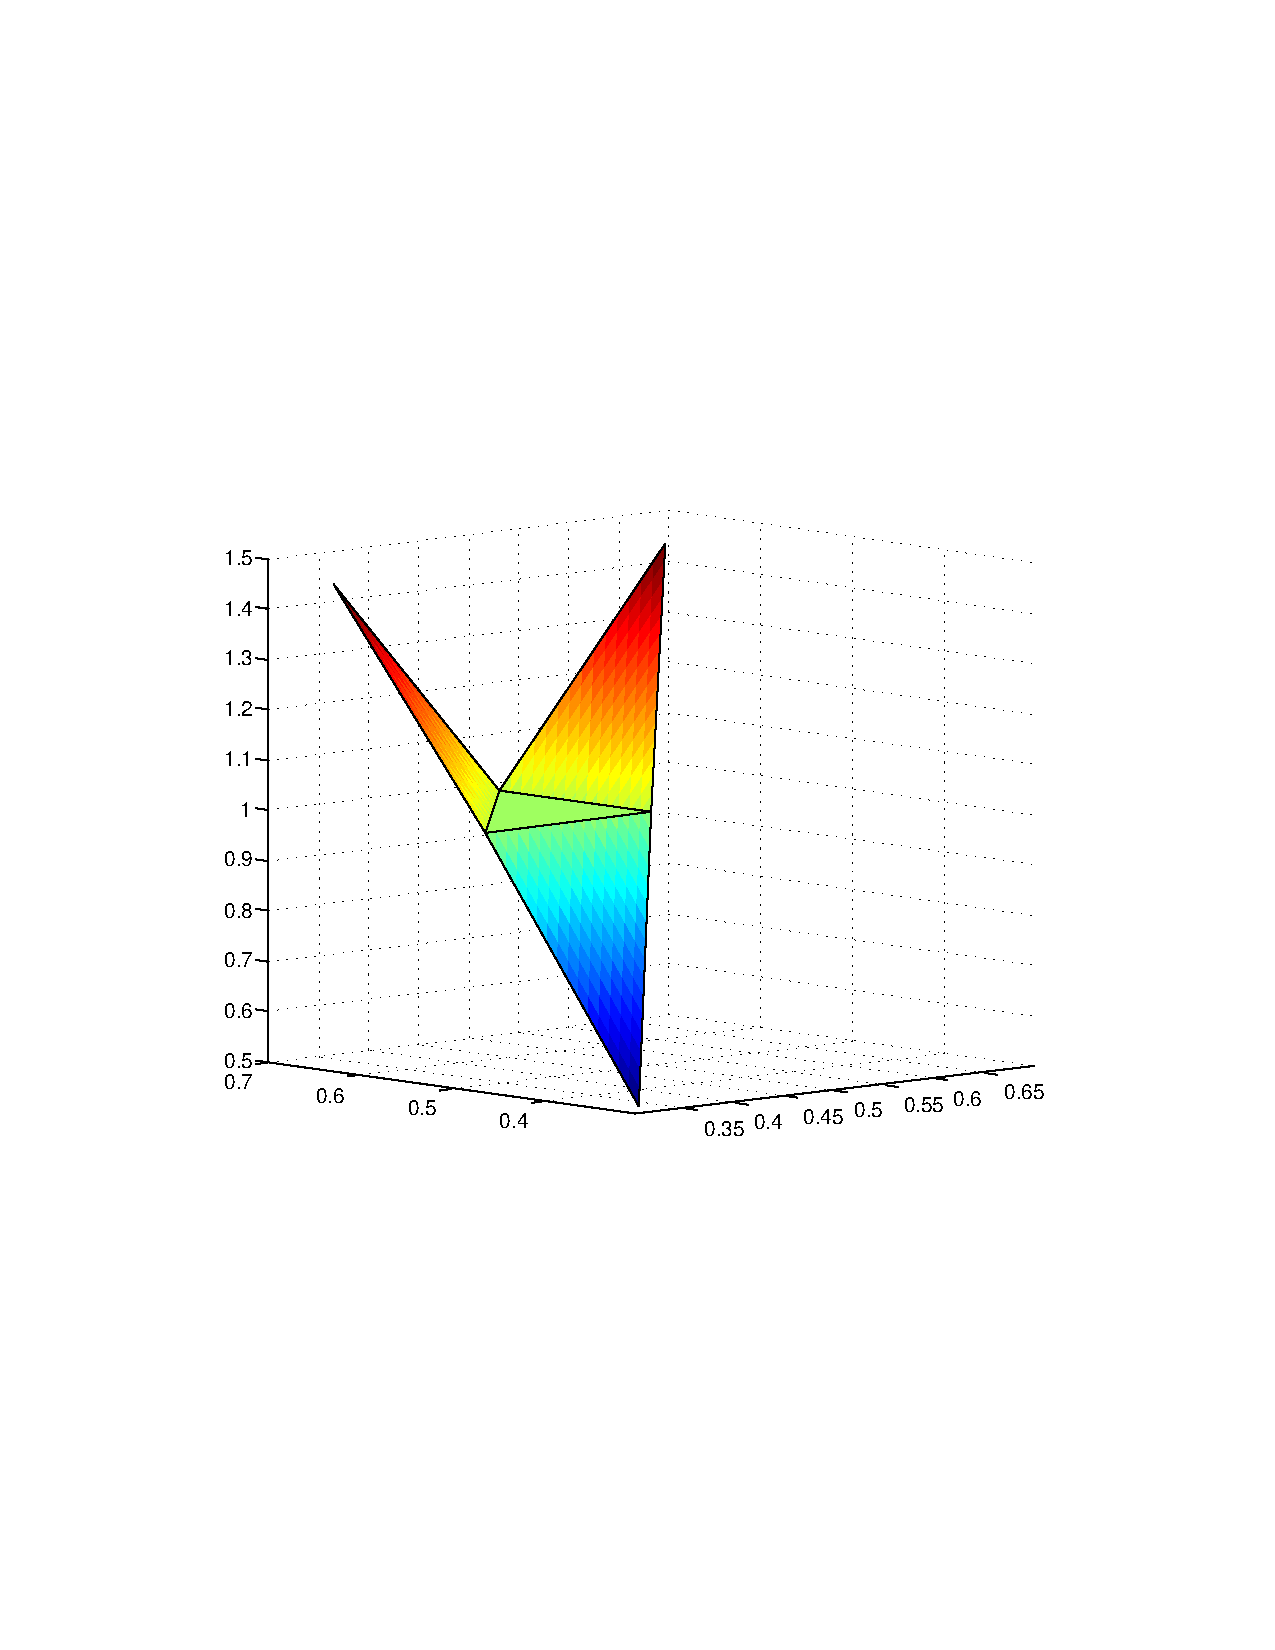
\includegraphics[trim=3cm 8cm 3cm 8cm, width=1.\textwidth]{control_polygon2.pdf}
	\caption{control polygon}
\end{subfigure}
\begin{subfigure}[b]{.5\textwidth}
	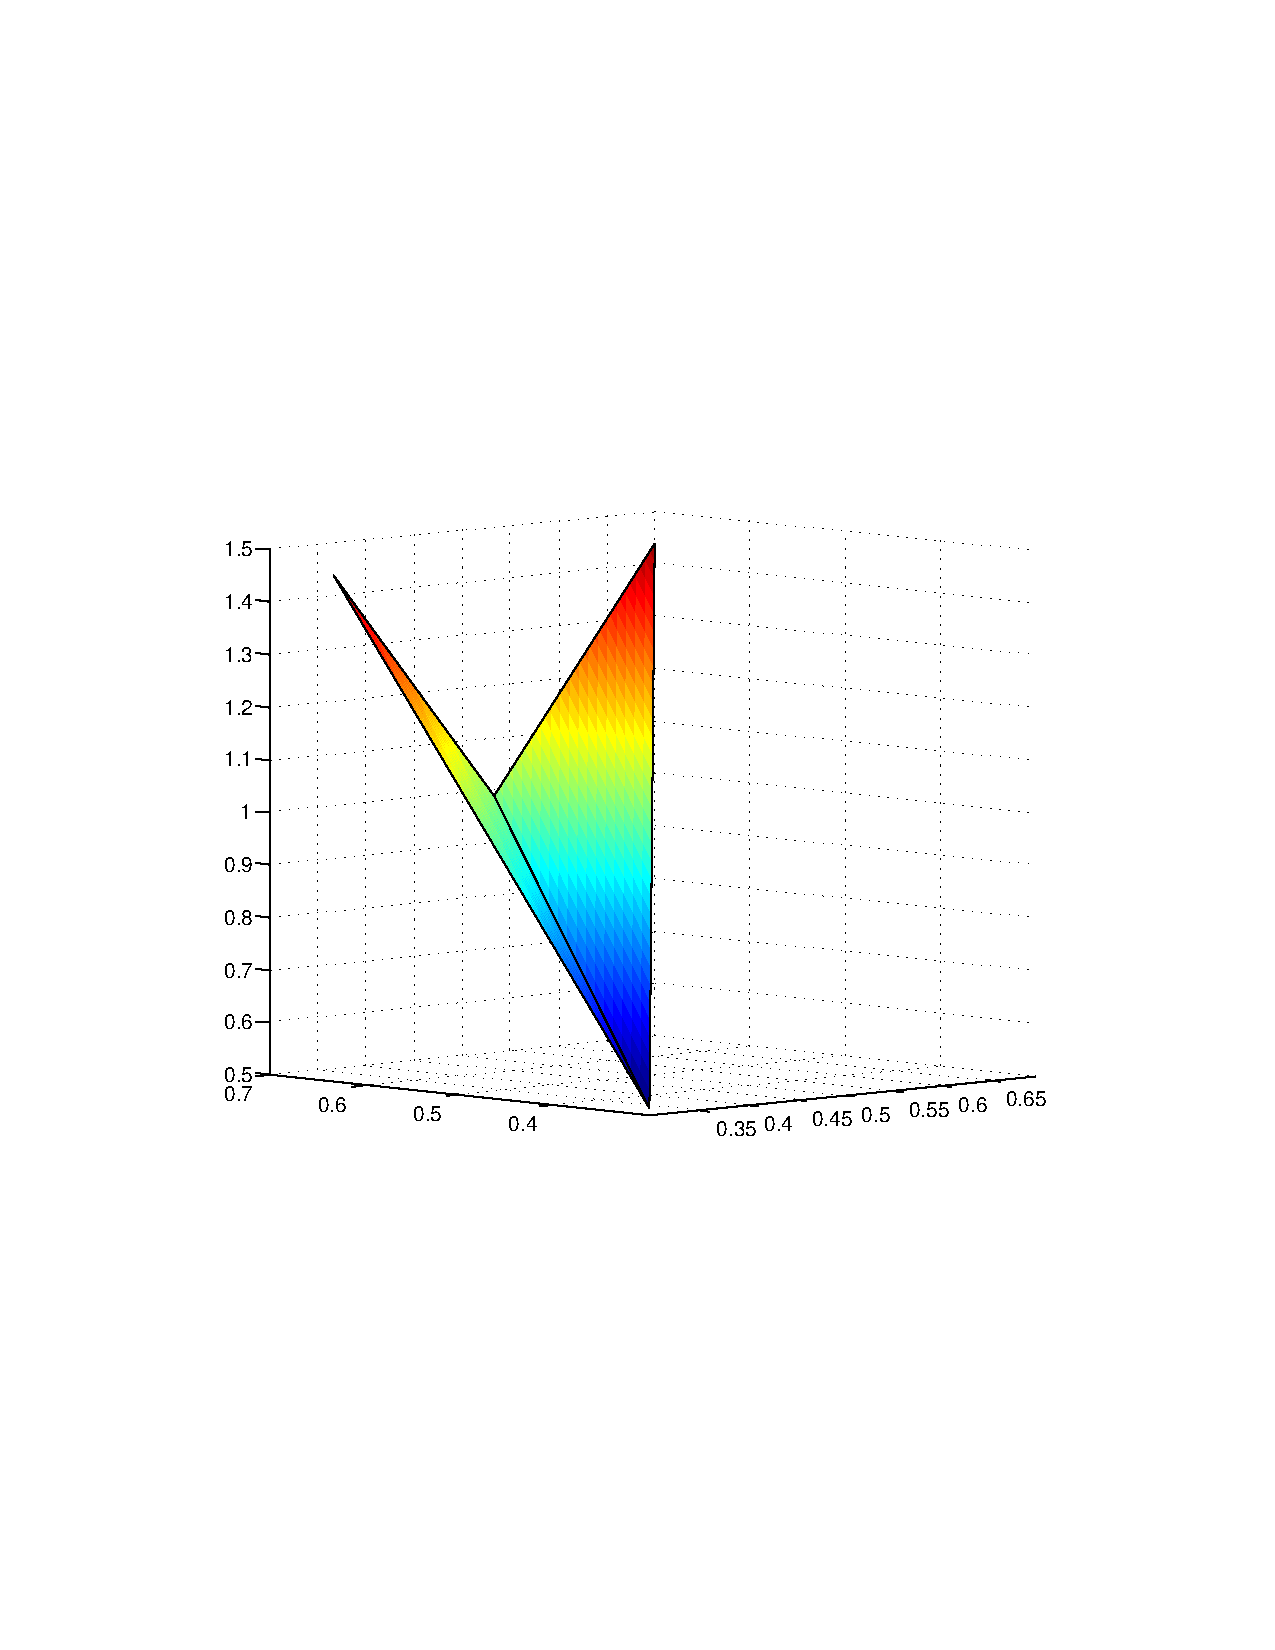
\includegraphics[trim=3cm 8cm 3cm 8cm, width=1.\textwidth]{convex_hull2.pdf}
	\caption{lower convex hull}
\end{subfigure}
\caption{The control polygon and lower convex hull of a given set of control points}
\label{fig: diff connectivity}
\end{figure}

While the the control polygon is obviously not convex, the surface of the lower convex hull of the control points is convex because it connect the inner control points differently.

Schumaker and Speleers present in \cite{SS2014} an approach to ensure convexity by a set of conditions on the coefficents , resulting in a quadratic program with linear constraints. To set up the convexity constraints we first need to define the difference operator
\begin{definition}[Difference Operator]
	$\Delta_{\mu \nu}$ is the \emph{difference operator} along the edge $(v_\mu, v_\nu)$ as for example
	\begin{align*}
		\Delta_{21} c_{ijk} &= c_{i,j+1,k} -c_{i+1, j,k}  \\
		\Delta_{31}^2 c_{ijk} &= c_{i,j,k+2} -2c_{i, j+1,k+1} +c_{i, j+2,k} \\
		\Delta_{12} \Delta_{32} c_{ijk} &= c_{i,j+1,k+1} -c_{i+1, j,k+1} - c_{i,j+2,k} +c_{i+1, j+1,k}\\	\end{align*}
\end{definition}
 
Lai and Schumaker present in \cite{LS2007} \todo{siehe nummer 3 in $C^0 $ schumaker paper} a sufficient condition to ensure convexity on a triangle.
\begin{theorem}[A Sufficient Condition for Convexity]
	A polynomial $p$ is convex on a triangle $T$ if the matrix
	\[
		\begin{pmatrix}
			\Delta_{21}^2 c_{ijk} & \Delta_{31} c_{ijk} \Delta_{32} c_{ijk}\\
			\Delta_{31}c_{ijk} \Delta_{32} c_{ijk} & \Delta_{31}^2 c_{ijk} 
		\end{pmatrix}
	\]
	is nonnegative definite for each $i + j + k =2 $.
\end{theorem}
Note, that this condition is quadratic in the coefficients. But there are many relaxations of these conditions, we refer the interested leader to \cite{SS2010}. \todo{zitate}An example with 12 inequalities is \todo{welche art von satz, theorem, etc?}
\begin{theorem}[Sufficient Linear Conditions for Convexity]
	A polynomial $p$ is convex on a triangle $T$ if its B\'ezier coefficient $c_{ijk}$ satisfy
	\begin{align*}
		&(\Delta_{21} + 2\Delta_{31}) \Delta_{31} c_{ijk} \geq 0, 
		&   (\Delta_{21}^2 + 3\Delta_{21} \Delta_{31} + 2 \Delta_{31}^2) c_{ijk} \geq 0, \\
		& \Delta_{21}(2\Delta_{21} + \Delta_{31})  c_{ijk} \geq 0, 
		&   (2\Delta_{21}^2 + 3\Delta_{21} \Delta_{31} +  \Delta_{31}^2) c_{ijk} \geq 0, \\  
		&(\Delta_{32} + 2\Delta_{12}) \Delta_{12} c_{ijk} \geq 0, 
		&   (\Delta_{32}^2 + 3\Delta_{32} \Delta_{12} + 2 \Delta_{12}^2) c_{ijk} \geq 0, \\
		&\Delta_{32} (2\Delta_{32} + \Delta_{12}) c_{ijk} \geq 0, 
		&   (2\Delta_{32}^2 + 3\Delta_{32} \Delta_{12} +  \Delta_{12}^2) c_{ijk} \geq 0, \\  
		&(\Delta_{13} + 2\Delta_{23}) \Delta_{23} c_{ijk} \geq 0, 
		&   (\Delta_{13}^2 + 3\Delta_{13} \Delta_{23} + 2 \Delta_{23}^2) c_{ijk} \geq 0, \\
		& \Delta_{13}(2\Delta_{13} + \Delta_{23})  c_{ijk} \geq 0, 
		&   (2\Delta_{13}^2 + 3\Delta_{13} \Delta_{23} +  \Delta_{23}^2) c_{ijk} \geq 0   
	\end{align*}
	for all $i + j + k =2 $.
\end{theorem}
The latter conditions only ensure convexity on a single triangle. That would suffice for piecewise polynomials contained $C^1$ because for them unlike to splines contained in $C^0$ convexity on each triangle implies global convexity. To patch this matter Schumaker and Speleers introduce further conditions making sure splines are convex across triangle boundaries//edges, as they prove in Theorem 3.6 \cite{SS2014}.
\begin{theorem}[Sufficient Conditions for Convexity across Triangle Edges]
	Let $p$ be a piecewise polynomial being convex on every triangle. Suppose its B\'ezier coefficients for every interior edge $e =(v_\kappa, v_\mu)$ fulfill 
	\begin{align}
		{\hat c_{i,j,1}} = \beta_1^c c_{i+1, 0,j} +\beta_2^c c_{i,1,j} + \beta_1^c c_{i, 0,j+1}, \; i+j=d-1, \label{eq: convexity across edge}
	\end{align}
where  $\{c_{i,j,k}\}_{i+j+k=d}$ and $\{ {\hat c_{i,j,k}}\}_{i+j+k=d}$ are the B\'ezier coefficients of $p$ relative to the two triangles $T_1 = \langle v_\kappa, v_\lambda, v_\mu \rangle$ and $T_2 = \langle v_\kappa, v_\mu, v_\nu \rangle$ sharing the edge $e$, and $(\beta_1^c,\beta_2^c,\beta_3^c)$ are the barycentric coordinates of $v_\nu$ with respect to $T_1$. Then $p$ is convex.
\end{theorem}

\begin{figure}[h]
			\begin{center}
		\begin{tikzpicture}
%define coordinates
			\coordinate (vEins) at (120:4cm) ;
			\coordinate (vZwei) at (60:4cm);
			\coordinate (vDrei) at (0:0cm);
			\coordinate (vVier) at (0:4cm);

			\draw (0,0) -- (vEins) -- (vZwei) -- node[above left ] {$e$} (vDrei) -- (vVier) -- (vZwei);

%draw nodes
			\draw[fill =black] (vEins) circle (1pt) node[left] {$ v_\nu$};
			\draw[fill =black] (vZwei) circle (1pt) node[right] {$v_\mu$};
			\draw[fill =black] (vDrei) circle (1pt) node[below] {$v_\kappa$};
			\draw[fill =black] (vVier) circle (1pt) node[right] {$v_\lambda$};

%draw control points in T_1
			\draw[fill =blue] ($(vEins)!0.5!(vZwei)$) circle (1pt) node[above] {$\blue{\hat \xi_{011}}$};
			\draw[fill =blue] ($(vEins)!0.5!(vDrei)$) circle (1pt) node[left] {$\blue{\hat \xi_{101}}$};
			\draw[fill =blue] ($(vDrei)!0.5!(vZwei)$) circle (1pt) node[left] {$\blue{\hat \xi_{110}}$};

			\draw[fill =blue] (vEins) circle (1pt) node[above] {$\blue{\hat \xi_{002}}$};
			\draw[fill =blue] (vZwei) circle (1pt) node[above] {$\blue{\hat \xi_{020}}$};
			\draw[fill =blue] (vDrei) circle (1pt) node[below left] {$\blue{\hat \xi_{200}}$};

%draw control points in T_2
			\draw[fill =blue] ($(vVier)!0.5!(vZwei)$) circle (1pt) node [right] {$\blue{\xi_{011}}$};
			\draw[fill =blue] ($(vVier)!0.5!(vDrei)$) circle (1pt) node[below] {$\blue{\xi_{110}}$};
			\draw[fill =blue] ($(vDrei)!0.5!(vZwei)$) circle (1pt) node[right] {$\blue{ \xi_{101}}$};

			\draw[fill =blue] (vZwei) circle (1pt) node[below right] {$\blue{\xi_{002}}$};
			\draw[fill =blue] (vDrei) circle (1pt) node[below right] {$\blue{\xi_{200}}$};
			\draw[fill =blue] (vVier) circle (1pt) node[below] {$\blue{ \xi_{020}}$};

			\draw node at (90:2.2cm) {$T_2$};
			\draw node at (30:2.4cm) {$T_1$};
			
		\end{tikzpicture}
		\end{center}

	\caption{Two triangles}
\end{figure}

For quadratic splines Schumaker and Speleers even prove the inversion on convex domains $\Omega$, namely if for every interior edge its coefficients satisfy \eqref{eq: convexity across edge} then the corresponding spline is convex.
This result does not generalise for higher degrees. In fact they give a counterexample for degree $k = 3$.

Now we apply the new insights//methods to the function given after solving the generalised poisson problem stated in \ref{?}.
Given the DG solution of the generalised poisson problem $u^{gp}_h$ we seek for a convex spline minimising the error at the B\'ezier control points, i.e. we want to find the B\'ezier coefficients $c$ minimising
\[
		\lVert A c - b \rVert_2, \qquad \text{ such that } Cc \geq 0,
\]
where $A$ is the matrix evaluating the to $c$ corresponding piecewise polynomial at the B\'ezier control points, $b$ are the function values of $u^{gp}_h$ at the B\'ezier control points and $C$ is the matrix containing the conditions ensuring convexity on the whole domain.

\subsubsection{Solving the Quadratic Program}
\todo{how to solve the quadratic program}

\subsection{Penalty Evaluation}

\subsection{Initial Guess}
Just as the most methods for the \MA equation the fixed point iteration requires an initial guess. Two approaches are very favoured in the literature.
One is to start with the solution of the equation
\begin{align}
	\begin{split}
	\triangledown u &= \sqrt{2f} \text{ in } \Omega \\ 
	u &= g \text{ on }\partial \Omega.
	\end{split}\label{eq: start sqrt_f}
\end{align}

\todo{motivation for this approach}

The other is a nested iteration ansatz. At a the coarsest level $h_1$ one chooses any convex function as initial guess$u^0_{h_1}$, mostly $\frac 1 2 ({x_1^2} + {x_2^2}) $ for it is convex polynomial with a low degree. For finer triangulations $\mathcal{T}_{h_{l}}$ the solution of the previously computed solution $u_{h_{l-1}}$is taken for a starting point.

Advantageously at the first approach is the compliance of the boundary conditions.
The second approach regards the fact that probably the method's robustness decreases for finer meshes.


\section{First Implementation}
At the beginning we implemented the SIPG method exactly as stated in section \ref{sec: SIPG}.
As an initial guess served the solution of \eqref{eq: start sqrt_f} , the penalty parameter was chosen to be 30 and the domain $\Omega$ the unit square$[0,1]^2$.

For first numerical results we consider the rather simple equation
\begin{align}
	\mydet {D^2 u} &= 1 \text{ in } \Omega \\ 
	u &= \frac 1 2 (x_1^2 + x_2^2 )\text{ on }\partial \Omega.	
\end{align}
with the exact classical solution $\frac 1 2 (x_1^2 + x_2^2 )$. However, even for this rather simple example the iteration does not converge. This implementation even fails the consistency check. Given the exact solution as starting point the $L2$ error steadily increases, as shown in figure \ref{fig: consisctency_first_try}
\begin{figure}[h]
	\centering
	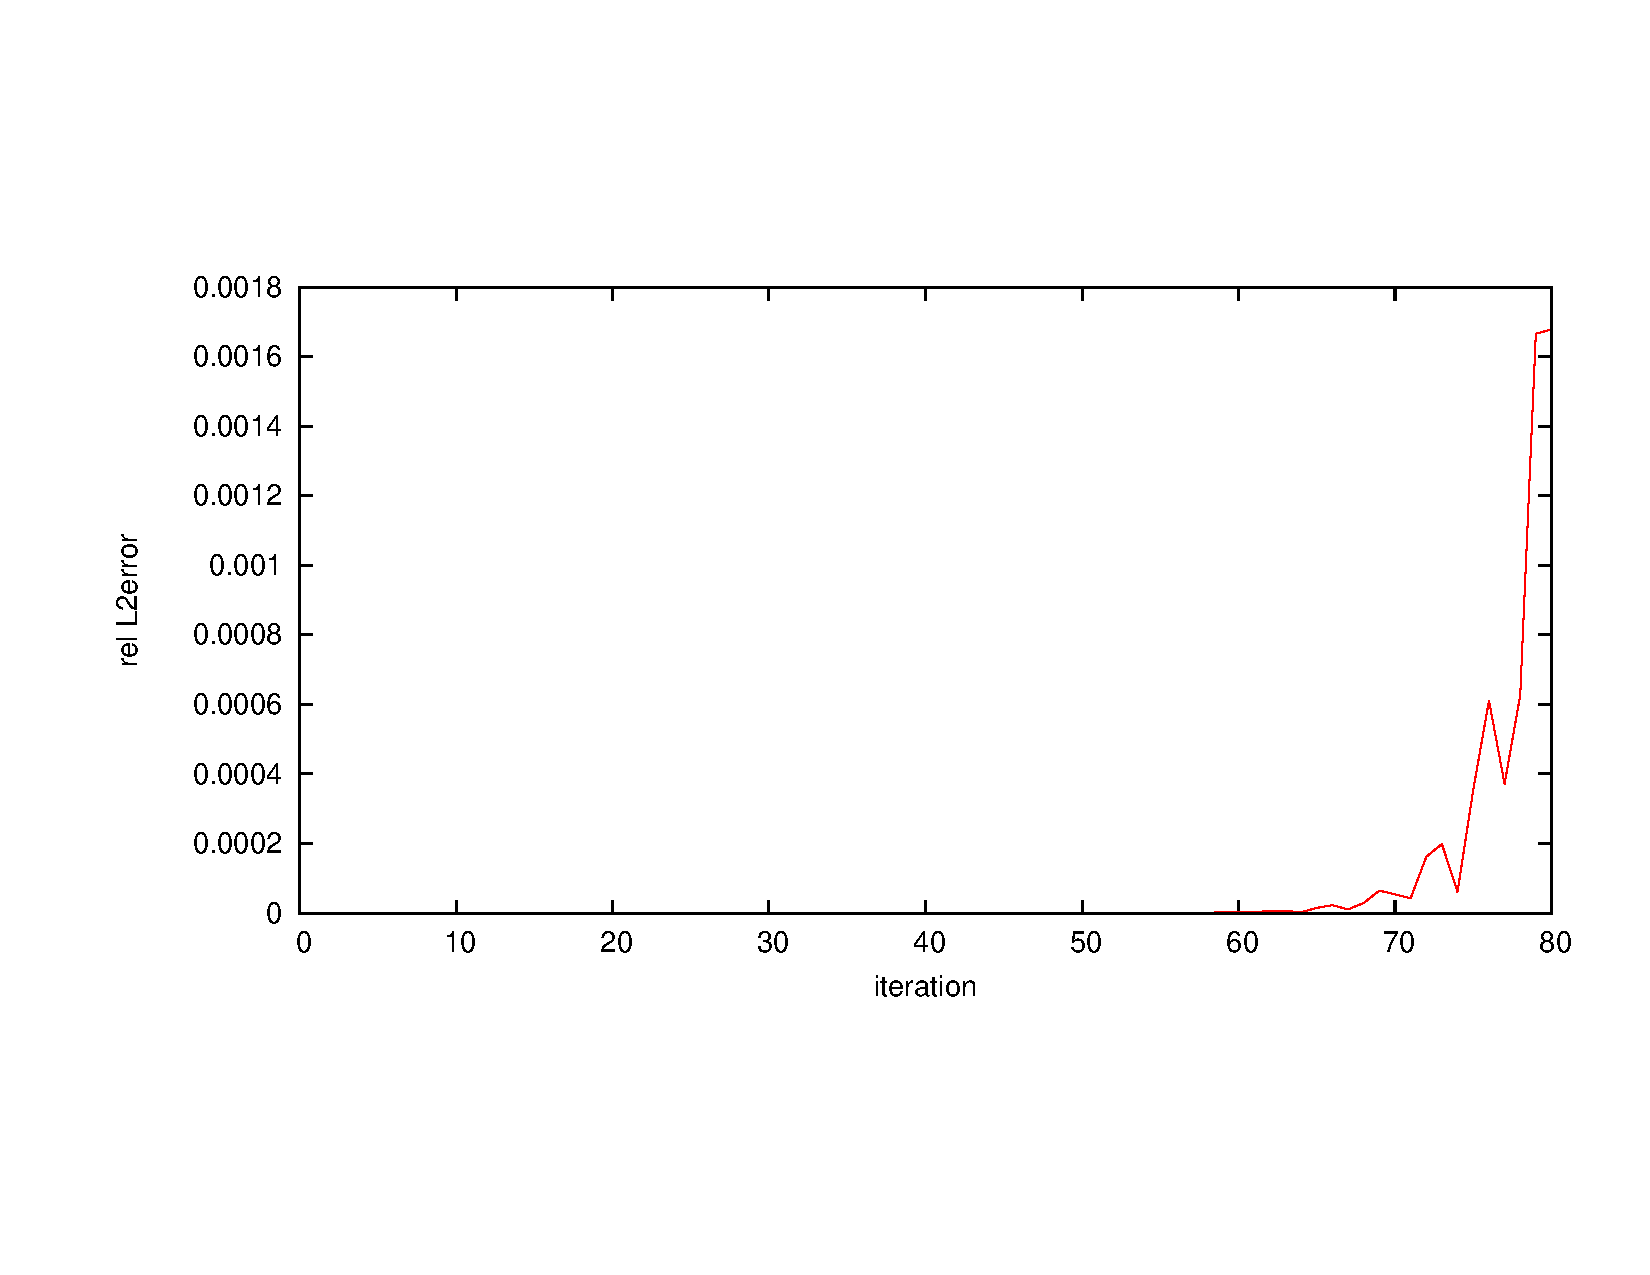
\includegraphics[trim = 2cm 4cm 1cm 4cm, width=1\textwidth]{plots/consisctency_first_try.pdf}
	\caption{Relative $L2$ error on a grid with $h=\frac 1 2$}
	\label{fig: consisctency_first_try}
\end{figure}
Looking at latter steps one is able see in the solution the underlying grid structure. Everywhere a triangle edge lies sharps edges arise. Besides continuity the solution on two triangles seem independent although the exact solution is absolutely  regular.

A similar approach works for quasilinear methods, so it is a good starting to analyse the main difference, i.e. the derivation in the iterated variable. This leads us to the question: How good serves the second derivative of the Poisson solution for an approximation of the exact second derivative?
We illustrate the significance of this question by a example
\begin{example}
	Let $\tilde u$ be an approximation of $u\in C^2(\R)$ with $u-\tilde u \in \bigO(h)$. Differentiating twice we are left with $\dxx{x} u(x)-\dxx{x} \tilde u(x)\in \bigO(h^{-1})$ meaning a decrease of the grid size comes along with a increase of the error in the second derivatives.
	????????//
	 an approximation find
	\begin{align*}
		\dxx{x} u(x)-\dxx{x} \tilde u(x) \approx \frac{\tilde u(x+2h) - 2\tilde u(x) - \tilde u(x-2h) - (u(x+2h) - 2u(x) - u(x-2h))} {4h^2} \\
		 \in \bigO(h^{-1})
	\end{align*}
\end{example}
Let us recall the geometric interpretation of the second derivative, it indicates the curvature of a function and hence also describes the convexity, concavity respectively.

In order to simplify the required calculation we restricted ourselves test space of piecewise polynomials of degree 2. Hence, we receive a piecewise constant Hessian in every step which is especially during the first iterations not smooth.
On one hand one can hope for a smoothing by a convexification for it will smooth away all unintended concave curvatures. But on the other hand the result is still unsatisfiable because convexification does not affect sharp edges at triangle transitions.

\subsection{An additional Penalty Parameter}
Another idea is force more regularity on the first derivative and thus, implicitly obtain a more steady solution. This suits to the ansatz pursued by Neilan described in section \ref{subsec: disrete Hessian}, his proposed correction terms vanish as the gradient jump across internal edges tends to zero.
Hence, we add the following normal derivatives penalty term 
\begin{align}
	\sum_{e \in \edgesi} \sigma_g |e |\int_e \jump{ \nabla u} \jump {\nabla v} \label{eq: grad penalty term}
\end{align}
to the formulation in \eqref{eq: sipg iteration}.
Note, that this is a strong demand on our solution. We implicitly imply that the desired solution is contained in $H^2(\Omega)$, it is not yet clear how this term behaves for less regular solution.
But, indeed with the new penalisation of the gradient the implementation is consistent with the previous example. The consistency check was carried out with the choice $\sigma_g$ equal to $\sigma=30$, as well as for much smaller choices.
\todo{Noelle gluecklich machen querschnitt}

Nevertheless, starting over with the initial guess from \eqref{eq: start sqrt_f} the method is instable and diverges. But the results yet are very remarkable. As shown in figure \ref{fig: oscillation} the error is oscillating while diverging  to infinity.
\begin{figure}[h]
	\centering
	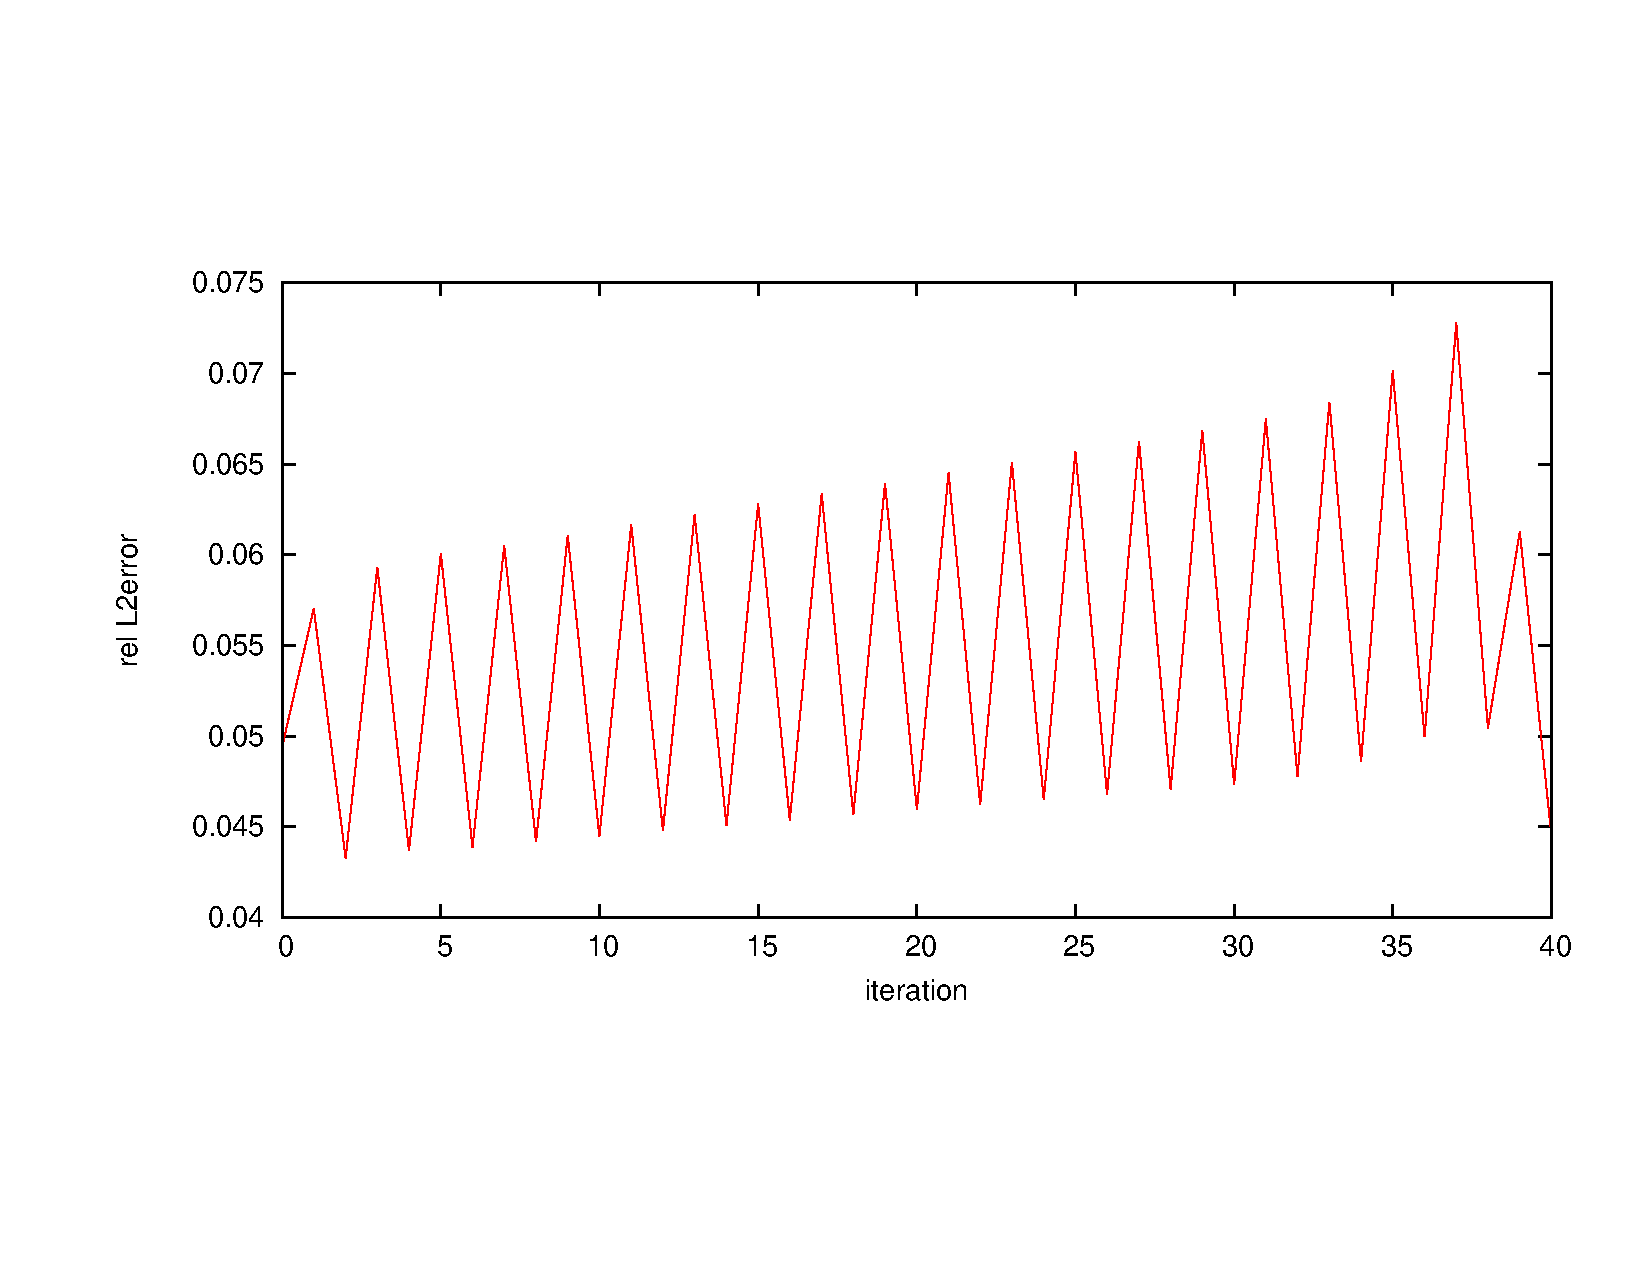
\includegraphics[trim = 2cm 4cm 1cm 4cm, width=1\textwidth]{plots/oscillation.pdf}
	\caption{Relative $L2$ error on a grid with $h=\frac 1 4$ and gradient penalty}
	\label{fig: oscillation}
\end{figure}

\begin{figure}[h]
\begin{subfigure}[b]{.5\textwidth}
	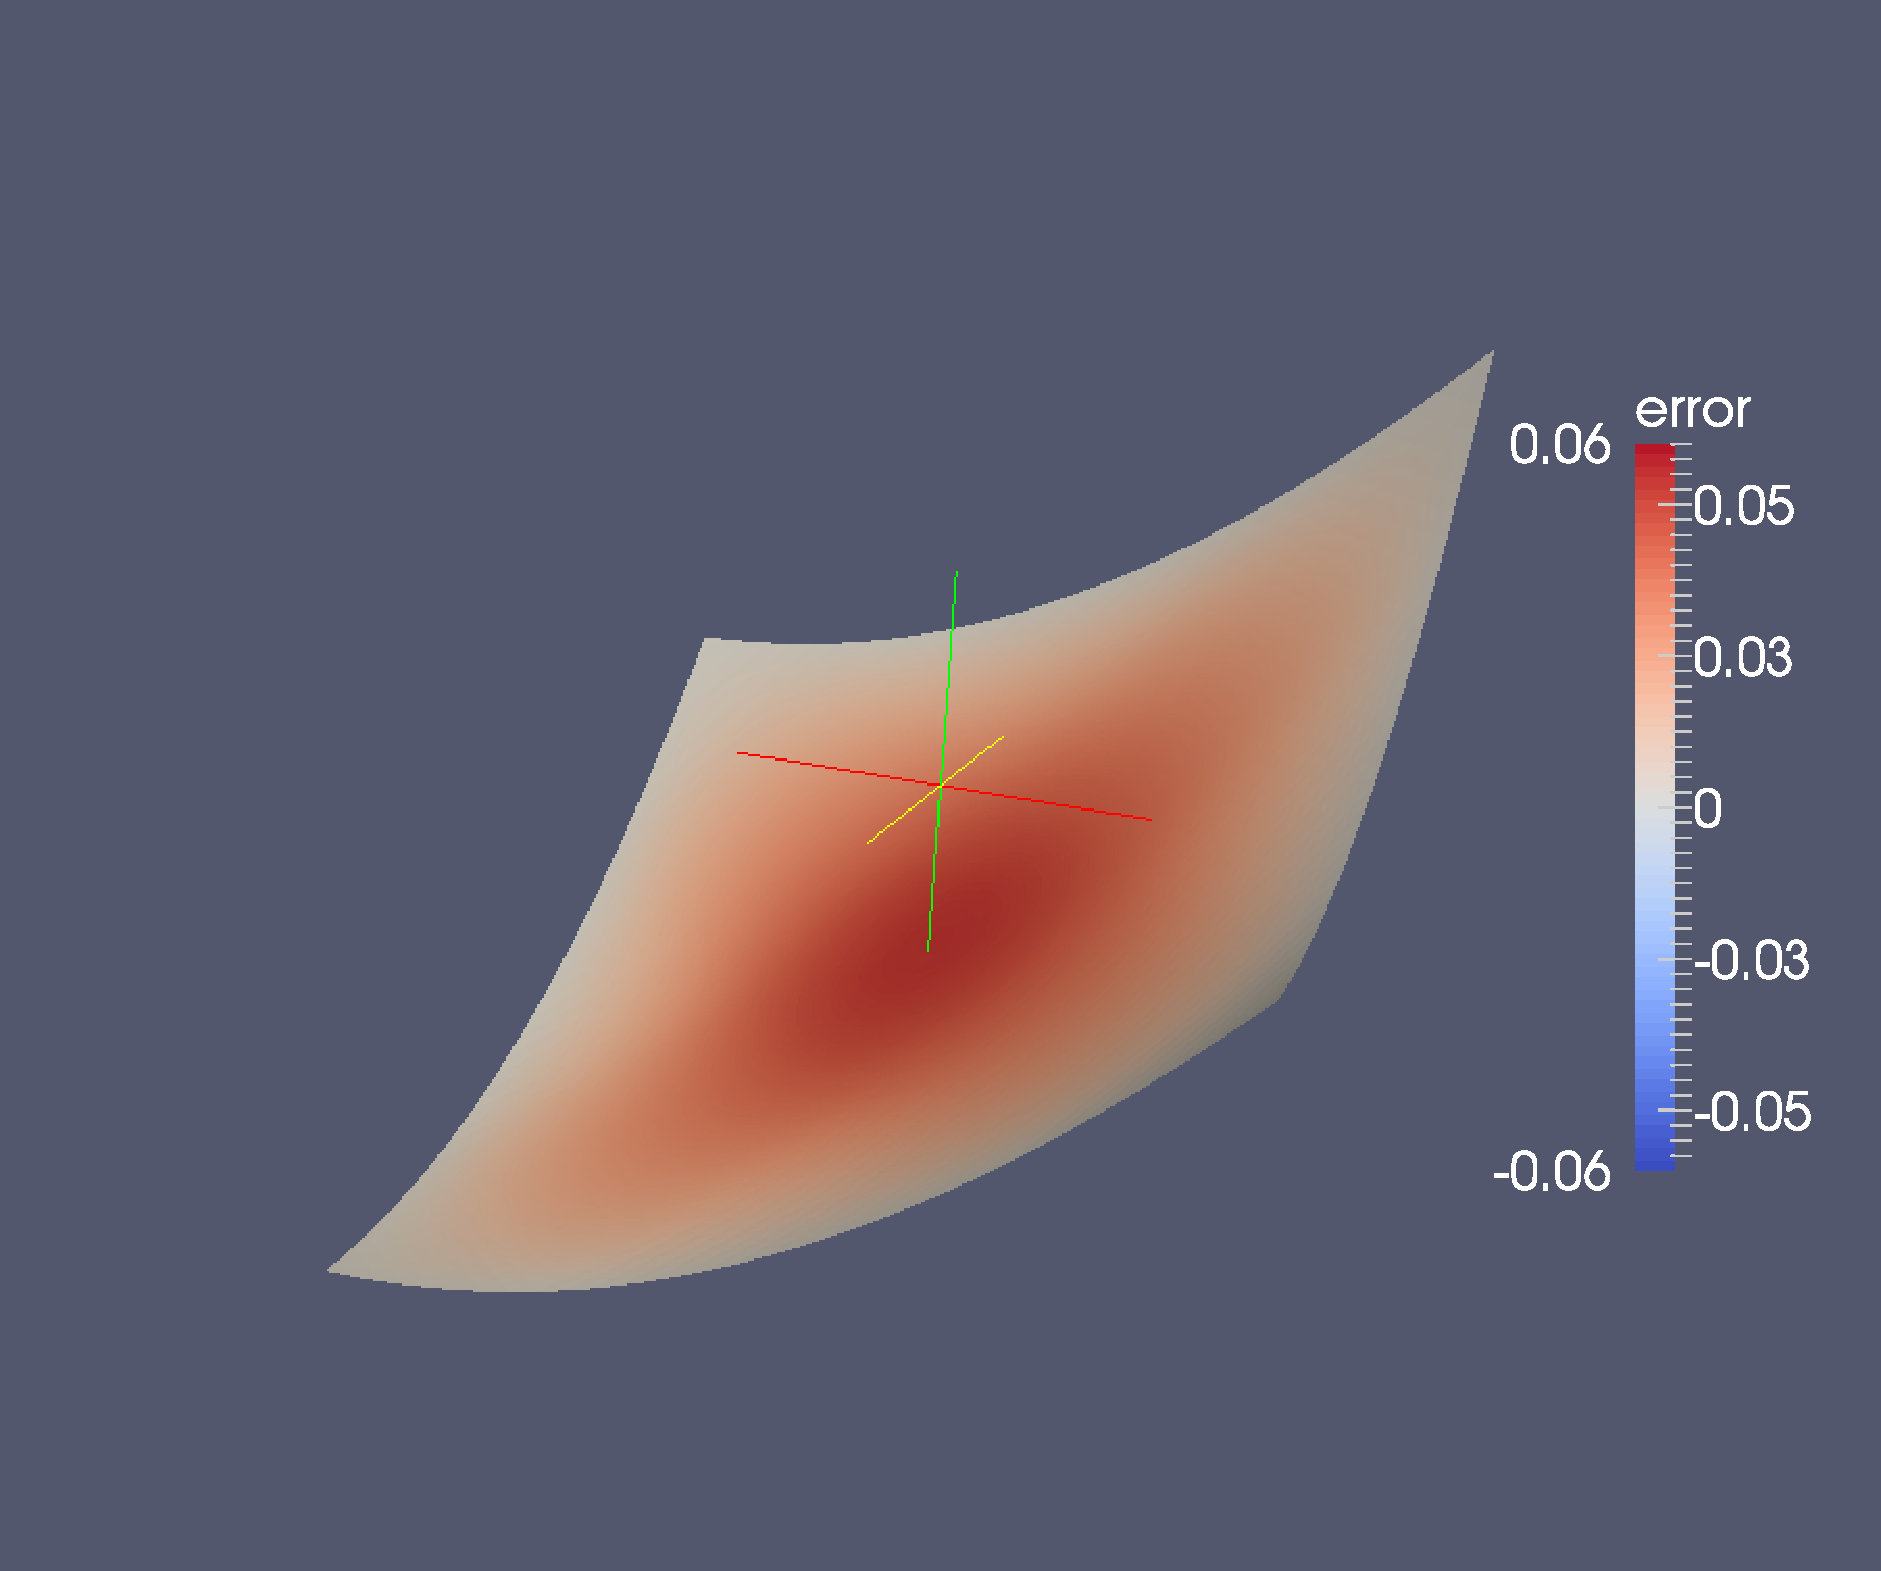
\includegraphics[width=1.\textwidth]{plots/with_penalty_it22.pdf}
	\caption{Solution after 23 steps}
\end{subfigure}
\begin{subfigure}[b]{.5\textwidth}
	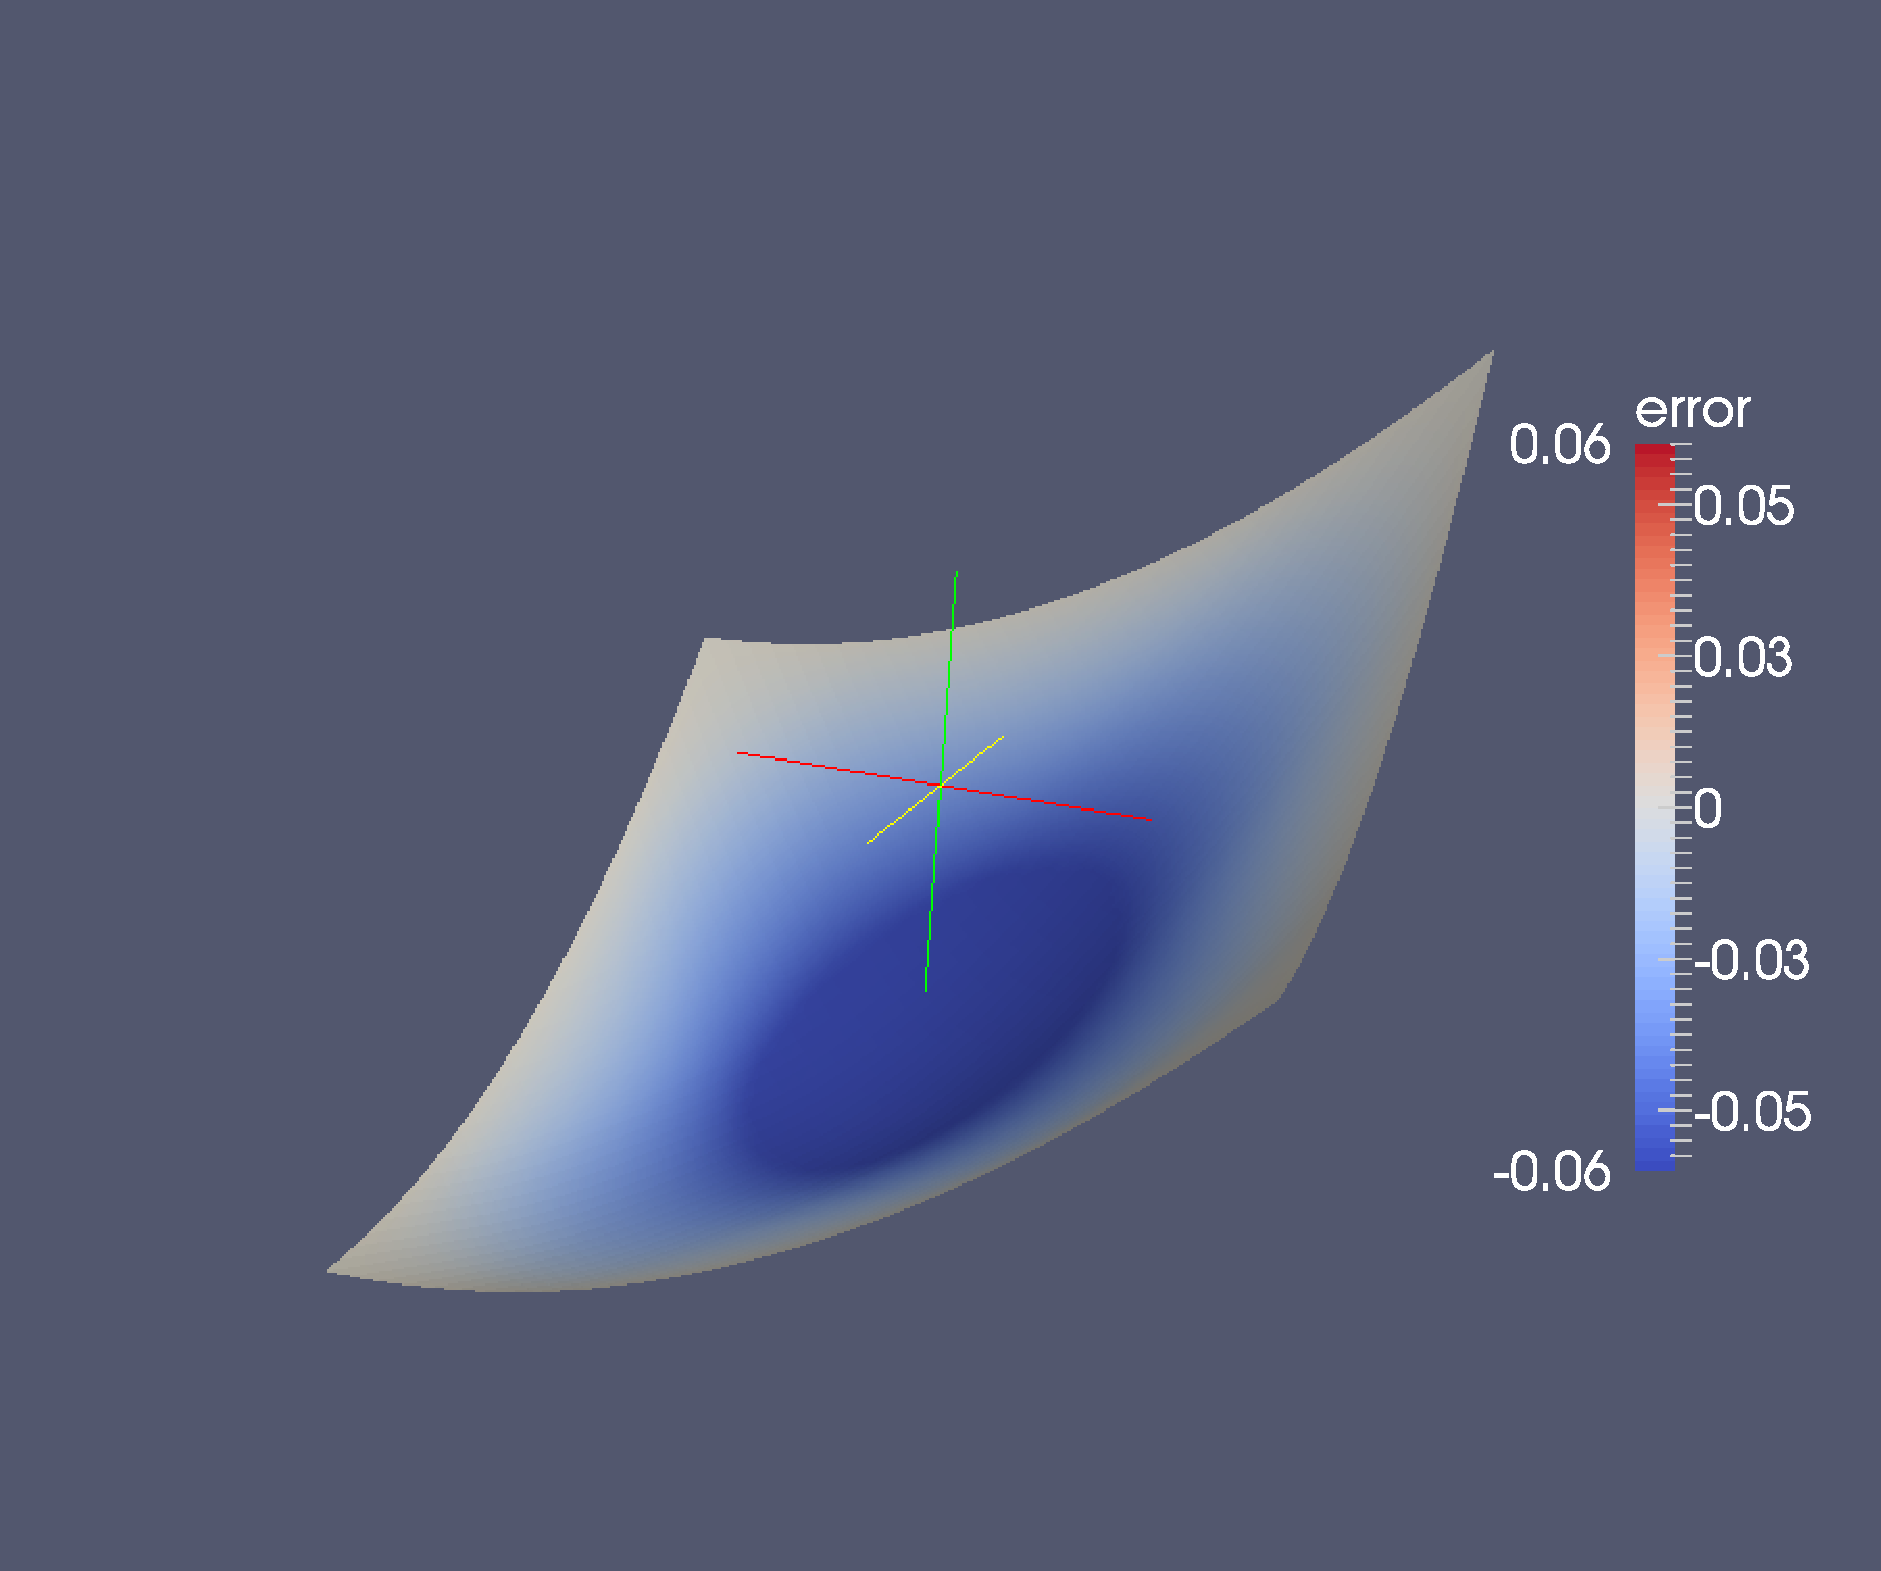
\includegraphics[width=1.\textwidth]{plots/with_penalty_it23.pdf}
	\caption{Solution after 24 steps}
\end{subfigure}
\caption{The solution in two consecutive iterations}
\label{fig: diff iteration}
\end{figure}
Figure \ref{fig: diff iteration} shows to consecutive steps, the error $u-u_{exact}$ is denoted by the surface color. We see that the solution after 23 steps lies above of the exact solution, while one iteration later the Poisson solution lies below of it. These frames are exemplary for the behaviour of our numerical solution. After a step above the solution one below follows, it looks like the solution is split into two subsequences.  And as we have also seen in the devolution of the error, these subsequences seem even to drive each other away from the actual solution.

To prevent our algorithm from doing so we couple the two subsequences by a damping. Before we continue iterating we combine the current solution with the function calculated one step before by an affine composition. Hence we got a further parameter $\alpha$, namely the amount with that the new solution contributes to the iteration.




\section{The final implementation}

\begin{algorithmic}
\State $u_0\gets $ solution of  $
	\triangle u = \sqrt{2f} \text{ in } \Omega $ with $
	u = g \text{ on }\partial \Omega$
\State $i \gets 1$
\While {$u_i-u_{i-1} < \varepsilon$}
	\State $u_i \gets$ solution of \ref{sec: SIPG}
	\State $u_i \gets \alpha u_{i-1} + (1-\alpha)u_i $
	\State convexify ??????????/
\EndWhile
\end{algorithmic}


